\documentclass{article}
\usepackage[backend=biber,style=authoryear]{biblatex}
\usepackage{graphicx}
\usepackage{caption}
\usepackage{geometry}
\usepackage{placeins}
\usepackage{enumitem}
\usepackage{tcolorbox}
\usepackage{multirow}
\usepackage{float}
\usepackage{hyperref}
\usepackage{tabularx}
\usepackage{tikz}
\usepackage{colortbl}
\usepackage{xcolor}
\definecolor{lightgray}{RGB}{245,245,245}


\addbibresource{references.bib}

% Set page margins
\geometry{a4paper, margin=2cm}

% Set paragraph spacing
\setlength{\parindent}{0em} % No indentation
\setlength{\parskip}{0.5em} % Space between paragraphs




\begin{document}

\title{PAR - Assignment 3 - Report}
\author{\normalsize Bruno Sánchez \& Jean Dié}
\date{\small 15th December 2024}

\maketitle

\newpage
\tableofcontents
\newpage

\section{Introduction}

% Introduce the problem of designing a fuzzy expert system to detect phishing on websites. Outline the objectives and significance of the project.

\section{Task 1: Definition of Linguistic Variables}\label{sec:task1}

In this task, we define the input and output linguistic variables for our fuzzy expert system designed to detect phishing on websites. Based on the features identified in \cite{Hannousse2020-eq}, we have selected a subset of five features, each with different reference scales and units, to serve as input variables. For each variable, we have determined the number of terms, labels, and corresponding fuzzy sets using trapezoidal membership function in the (a, b, c, d) format, ensuring they satisfy the property of Fuzzy Partition.


\subsection{Input Linguistic Variables}

For our fuzzy phishing detection system, we have carefully selected five input linguistic variables that capture key characteristics of websites commonly exploited in phishing attacks. Each variable represents a different aspect of website legitimacy, from structural elements to reputation indicators. The variables have been chosen to provide complementary signals while maintaining interpretability. We specifically selected non-binary features because binary features cannot be effectively represented using triangular or trapezoidal membership functions.

\subsubsection{Ratio of Null Hyperlinks}
The variable f60 measures the percentage of non-functional or empty links within a webpage. As identified in \cite{Hannousse2020-eq}, this feature is particularly significant for phishing detection as it reflects both the structural integrity and maintenance quality of a website. Legitimate websites typically maintain their hyperlinks carefully, while phishing sites often contain numerous broken or placeholder links due to hasty creation or poor maintenance. The range spans from 0 to 100 percent and is characterized by three linguistic terms with trapezoidal membership functions:

\begin{table}[H]
\centering
\begin{tabularx}{\textwidth}{|>{\hsize=0.7\hsize}X|>{\hsize=0.6\hsize}X|>{\hsize=1.7\hsize}X|}
\hline
\textbf{Linguistic Term} & \textbf{Range} & \textbf{Argumentation} \\
\hline
Low & [0, 0, 15, 25] & Typical of legitimate websites with properly maintained links. A low ratio of null hyperlinks suggests that the website is well-maintained and regularly updated, reducing the likelihood of it being a phishing site. \\
\hline
Moderate & [15, 25, 35, 45] & Indicates potential suspicious activity. A moderate ratio of null hyperlinks may suggest that the website has some issues with link maintenance, which could be a sign of a less reputable site or one that is not regularly updated. \\
\hline
High & [35, 45, 100, 100] & Strong indicator of a phishing webpage. A high ratio of null hyperlinks is a red flag, as it suggests that the website may have been hastily created with little regard for link validity, a common trait of phishing sites. \\
\hline
\end{tabularx}
\caption{Linguistic Terms for Ratio of Null Hyperlinks}
\label{tab:null_hyperlinks}
\end{table}

\begin{figure}[H]
\centering
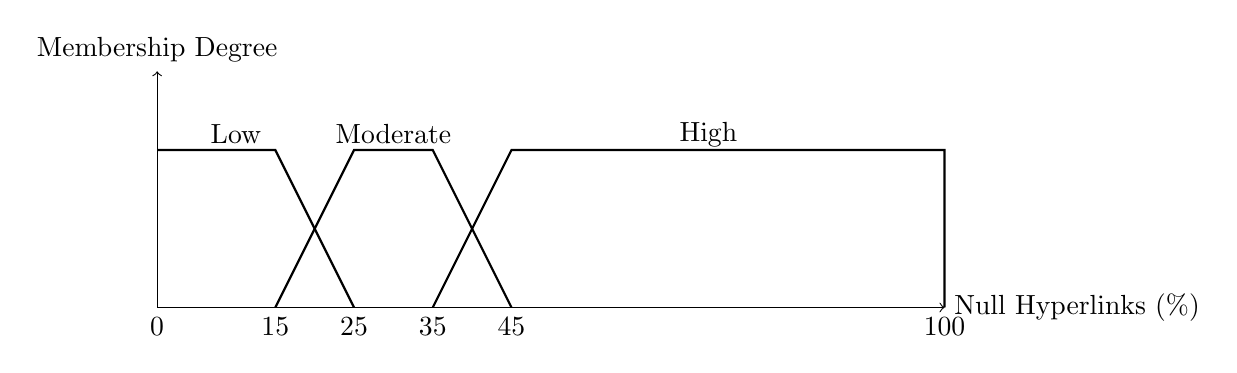
\begin{tikzpicture}
% Axis
\draw[->] (0,0) -- (10,0) node[right] {Null Hyperlinks (\%)};
\draw[->] (0,0) -- (0,3) node[above] {Membership Degree};
% Low
\draw[thick] (0,2) -- (1.5,2) -- (2.5,0);
\node at (1,2.2) {Low};
% Moderate
\draw[thick] (1.5,0) -- (2.5,2) -- (3.5,2) -- (4.5,0);
\node at (3,2.2) {Moderate};
% High
\draw[thick] (3.5,0) -- (4.5,2) -- (10,2) -- (10,0);
\node at (7,2.2) {High};
% Labels
\node[below] at (0,0) {0};
\node[below] at (1.5,0) {15};
\node[below] at (2.5,0) {25};
\node[below] at (3.5,0) {35};
\node[below] at (4.5,0) {45};
\node[below] at (10,0) {100};
\end{tikzpicture}
\caption{Membership Functions for Ratio of Null Hyperlinks}
\label{fig:membership_null_hyperlinks}
\end{figure}

\subsubsection{Number of External CSS Files}

The variable f61 quantifies external stylesheet references in a webpage. This feature is particularly relevant for phishing detection as legitimate websites typically maintain consistent styling through multiple CSS files, following modern web development practices. Phishing websites, in contrast, often minimize their styling implementation to quickly replicate legitimate pages with minimal effort. Additionally, as noted in \cite{10049452}, the number of external stylesheets can indicate the level of sophistication and development effort invested in the website, where an unusually low number might signal a hastily created phishing page. The range spans from 0 to 20 files, with three linguistic terms:

\begin{table}[H]
\centering
\begin{tabularx}{\textwidth}{|>{\hsize=0.7\hsize}X|>{\hsize=0.6\hsize}X|>{\hsize=1.7\hsize}X|}
\hline
\textbf{Linguistic Term} & \textbf{Range} & \textbf{Argumentation} \\
\hline
Very Few & [0, 0, 1, 2] & Common in phishing sites that employ minimal styling to create basic replicas of legitimate pages. A single CSS file often indicates oversimplified implementation that warrants scrutiny. \\
\hline
Few & [1, 2, 4, 5] & Represents balanced styling implementation. This range aligns with modern web development practices where CSS is modular but optimized for performance. \\
\hline
Normal & [4, 5, 20, 20] & Characteristic of properly developed sites with comprehensive styling needs. The upper limit reflects current best practices in CSS organization while acknowledging that excessive CSS files may indicate poor optimization. \\
\hline
\end{tabularx}
\caption{Linguistic Terms for Number of External CSS Files}
\label{tab:css_files}
\end{table}

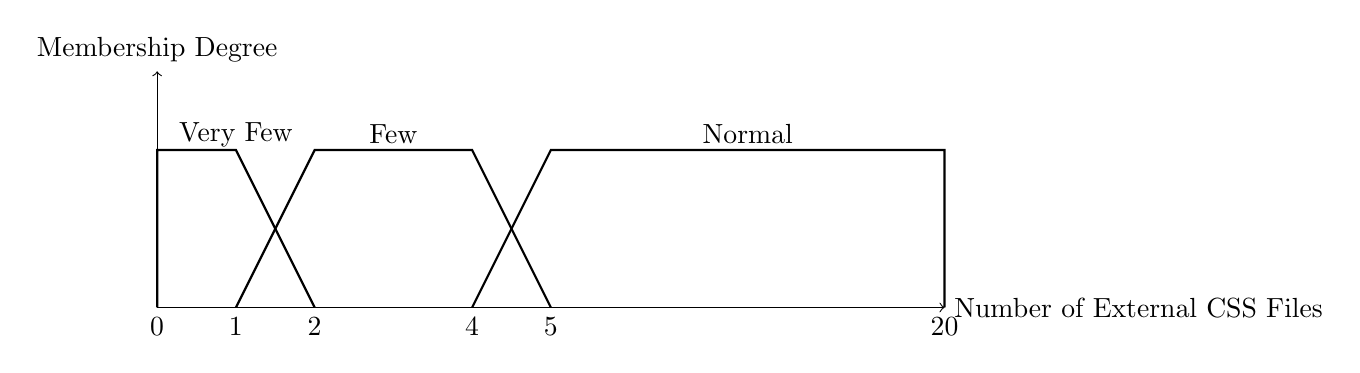
\begin{tikzpicture}
    % Axis
    \draw[->] (0,0) -- (10,0) node[right] {Number of External CSS Files};
    \draw[->] (0,0) -- (0,3) node[above] {Membership Degree};
    % Very Few
    \draw[thick] (0,0) -- (0,2) -- (1,2) -- (2,0);
    \node at (1,2.2) {Very Few};
    % Few
    \draw[thick] (1,0) -- (2,2) -- (4,2) -- (5,0);
    \node at (3,2.2) {Few};
    % Normal
    \draw[thick] (4,0) -- (5,2) -- (10,2) -- (10,0);
    \node at (7.5,2.2) {Normal};
    % Labels
    \node[below] at (0,0) {0};
    \node[below] at (1,0) {1};
    \node[below] at (2,0) {2};
    \node[below] at (4,0) {4};
    \node[below] at (5,0) {5};
    \node[below] at (10,0) {20};
\end{tikzpicture}

\subsubsection{Domain Registration Length}

The variable f82 reflects the duration of domain registration in years. According to \cite{8036198}, domain registration length is a crucial temporal feature for phishing detection, as legitimate websites tend to be registered for longer periods while phishing domains are typically short-lived. As noted in \cite{10049452}, attackers often register domains for the minimum required period to minimize costs and avoid detection, making registration length a strong indicator of potentially malicious intent. This pattern emerges because phishing campaigns are typically brief, targeted operations that don't require long-term domain maintenance. The range spans from 1 to 10 years and is characterized by the following:

\begin{table}[H]
\centering
\begin{tabularx}{\textwidth}{|>{\hsize=0.7\hsize}X|>{\hsize=0.6\hsize}X|>{\hsize=1.7\hsize}X|}
\hline
\textbf{Linguistic Term} & \textbf{Range} & \textbf{Argumentation} \\
\hline
Short & [1, 1, 2, 3] & Common for phishing domains. Short registration lengths are often used by phishing sites to avoid detection and minimize costs. \\
\hline
Medium & [2, 3, 5, 7] & Moderate commitment to domain maintenance. Medium registration lengths may indicate a more established site, but not necessarily a highly reputable one. \\
\hline
Long & [5, 7, 10, 10] & Typical of established legitimate websites. Long registration lengths suggest a strong commitment to maintaining the domain, which is characteristic of legitimate websites. \\
\hline
\end{tabularx}
\caption{Linguistic Terms for Domain Registration Length}
\label{tab:domain_registration_length}
\end{table}

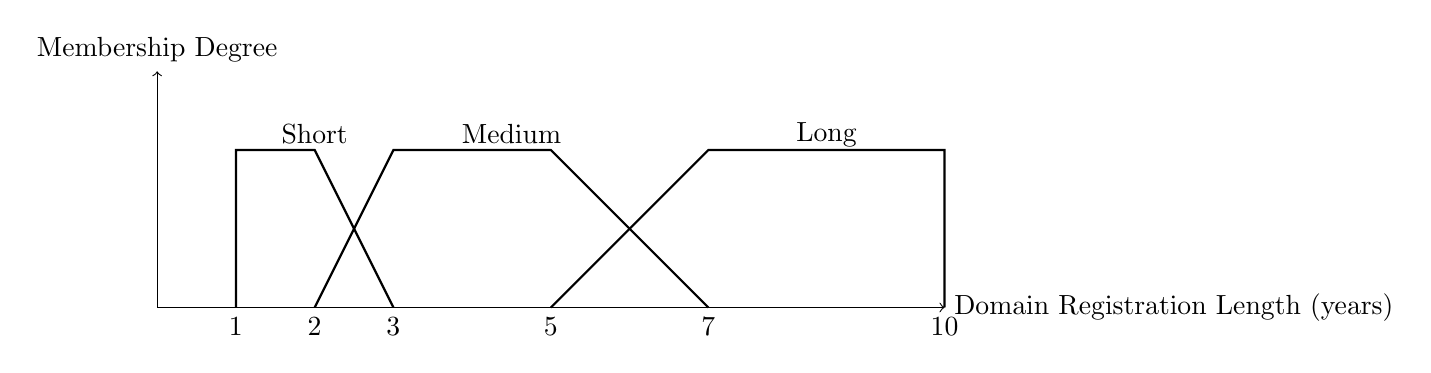
\begin{tikzpicture}
    % Axis
    \draw[->] (0,0) -- (10,0) node[right] {Domain Registration Length (years)};
    \draw[->] (0,0) -- (0,3) node[above] {Membership Degree};

    % Short
    \draw[thick] (1,0) -- (1,2) -- (2,2) -- (3,0);
    \node at (2,2.2) {Short};

    % Medium
    \draw[thick] (2,0) -- (3,2) -- (5,2) -- (7,0);
    \node at (4.5,2.2) {Medium};

    % Long
    \draw[thick] (5,0) -- (7,2) -- (10,2) -- (10,0);
    \node at (8.5,2.2) {Long};

    % Labels
    \node[below] at (1,0) {1};
    \node[below] at (2,0) {2};
    \node[below] at (3,0) {3};
    \node[below] at (5,0) {5};
    \node[below] at (7,0) {7};
    \node[below] at (10,0) {10};
\end{tikzpicture}

\subsubsection{Web Traffic}

The variable f84 measures the percentile rank of a website's traffic. Web traffic is a significant indicator of website legitimacy as it reflects the site's established presence and user trust. As noted in \cite{10049452}, phishing websites typically exhibit very low traffic patterns due to their short lifespan and targeted nature, while legitimate websites maintain consistent traffic levels over time. This metric is particularly valuable because it's difficult for attackers to artificially inflate genuine user traffic, making it a reliable indicator of legitimacy. The range spans from 0 to 100 percentiles and is characterized by four linguistic terms with trapezoidal membership functions:


\begin{table}[H]
\centering
\begin{tabularx}{\textwidth}{|>{\hsize=0.7\hsize}X|>{\hsize=0.6\hsize}X|>{\hsize=1.7\hsize}X|}
\hline
\textbf{Linguistic Term} & \textbf{Range} & \textbf{Argumentation} \\
\hline
Very Low & [0, 0, 10, 20] & Indicative of low visibility and potential risk. Websites with very low traffic are less likely to be well-known and may be newly created or less reputable. \\
\hline
Low & [10, 20, 60, 70] & Suggests limited reach and moderate risk. Low traffic websites may be legitimate but are not widely recognized, which can be a characteristic of less established sites. \\
\hline
Moderate & [60, 70, 80, 90] & Represents average visibility and lower risk. Moderate traffic websites are more likely to be established and have a consistent user base, indicating a higher likelihood of legitimacy. \\
\hline
High & [80, 90, 100, 100] & Characteristic of popular and reputable websites. High traffic websites are well-known and widely visited, reducing the likelihood of them being phishing sites. \\
\hline
\end{tabularx}
\caption{Linguistic Terms for Web Traffic}
\label{tab:web_traffic}
\end{table}

\begin{figure}[H]
\centering
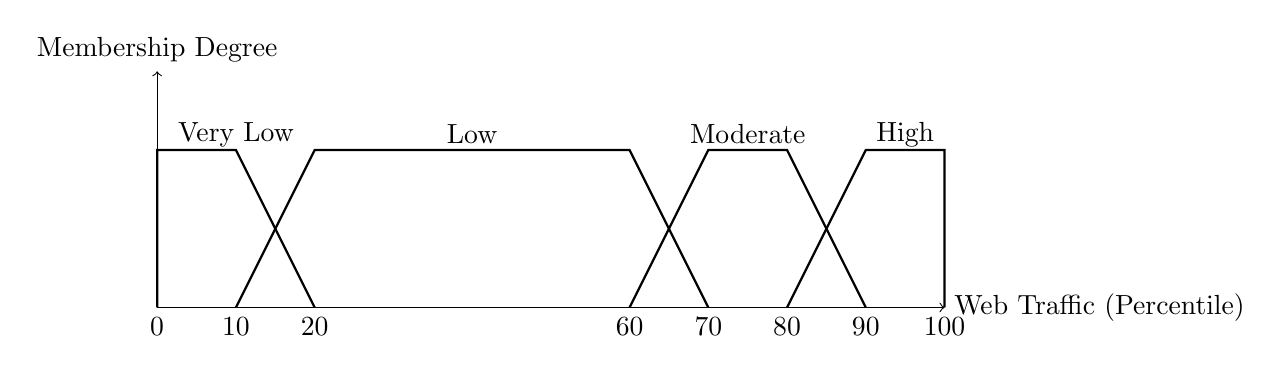
\begin{tikzpicture}
    % Axis
    \draw[->] (0,0) -- (10,0) node[right] {Web Traffic (Percentile)};
    \draw[->] (0,0) -- (0,3) node[above] {Membership Degree};

    % Very Low
    \draw[thick] (0,0) -- (0,2) -- (1,2) -- (2,0);
    \node at (1,2.2) {Very Low};

    % Low
    \draw[thick] (1,0) -- (2,2) -- (6,2) -- (7,0);
    \node at (4,2.2) {Low};

    % Moderate
    \draw[thick] (6,0) -- (7,2) -- (8,2) -- (9,0);
    \node at (7.5,2.2) {Moderate};

    % High
    \draw[thick] (8,0) -- (9,2) -- (10,2) -- (10,0);
    \node at (9.5,2.2) {High};

    % Labels
    \node[below] at (0,0) {0};
    \node[below] at (1,0) {10};
    \node[below] at (2,0) {20};
    \node[below] at (6,0) {60};
    \node[below] at (7,0) {70};
    \node[below] at (8,0) {80};
    \node[below] at (9,0) {90};
    \node[below] at (10,0) {100};
\end{tikzpicture}
\caption{Membership Functions for Web Traffic}
\label{fig:membership_web_traffic}
\end{figure}

\subsubsection{Page Rank}

The variable f87 measures the popularity score of a website, ranging from 0 to 10. This feature is meaninglful for phishing detection as it quantifies a website's reputation based on its relationships with other sites across the internet. While legitimate websites naturally accumulate higher page ranks through genuine backlinks and long-term presence, phishing sites typically have very low page ranks due to their recent creation and lack of legitimate connections. Unlike many other metrics, page rank is particularly difficult to manipulate as it requires building a genuine network of trusted referring sites. The range spans from 0 to 10 and is characterized by three linguistic terms with trapezoidal membership functions:

\begin{table}[H]
\centering
\begin{tabularx}{\textwidth}{|>{\hsize=0.7\hsize}X|>{\hsize=0.6\hsize}X|>{\hsize=1.7\hsize}X|}
\hline
\textbf{Linguistic Term} & \textbf{Range} & \textbf{Argumentation} \\
\hline
Popular & [0, 0, 2, 3] & Indicative of highly reputable websites. A high page rank suggests that the website is well-known and widely trusted, reducing the likelihood of it being a phishing site. \\
\hline
Moderately Known & [2, 3, 5, 7] & Represents websites with moderate popularity. These sites are somewhat known and trusted, but not as widely recognized as those with higher page ranks. \\
\hline
Not Very Known & [5, 7, 10, 10] & Characteristic of less reputable websites. A low page rank indicates that the website is not widely known or trusted, which could be a sign of a phishing site. \\
\hline
\end{tabularx}
\caption{Linguistic Terms for Page Rank}
\label{tab:page_rank}
\end{table}

\begin{figure}[H]
\centering
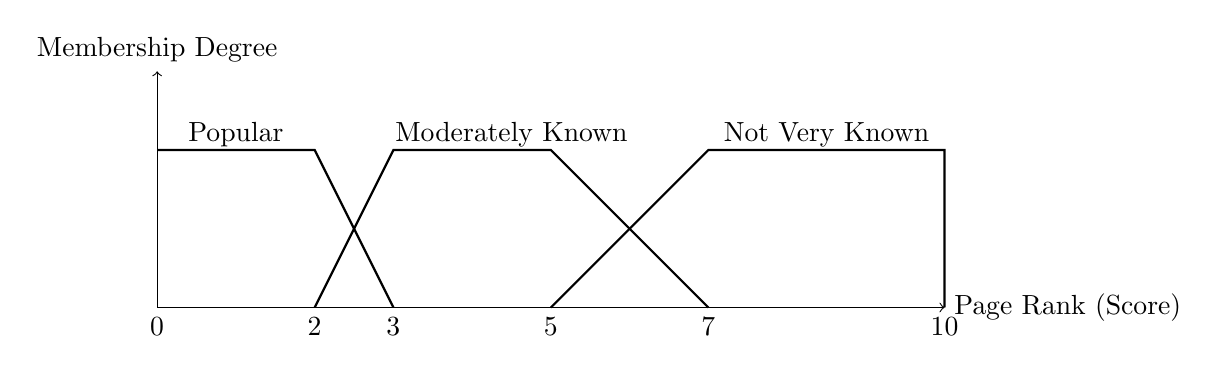
\begin{tikzpicture}
    % Axis
    \draw[->] (0,0) -- (10,0) node[right] {Page Rank (Score)};
    \draw[->] (0,0) -- (0,3) node[above] {Membership Degree};

    % Popular
    \draw[thick] (0,2) -- (2,2) -- (3,0);
    \node at (1,2.2) {Popular};

    % Moderately Known
    \draw[thick] (2,0) -- (3,2) -- (5,2) -- (7,0);
    \node at (4.5,2.2) {Moderately Known};

    % Not Very Known
    \draw[thick] (5,0) -- (7,2) -- (10,2) -- (10,0);
    \node at (8.5,2.2) {Not Very Known};

    % Labels
    \node[below] at (0,0) {0};
    \node[below] at (2,0) {2};
    \node[below] at (3,0) {3};
    \node[below] at (5,0) {5};
    \node[below] at (7,0) {7};
    \node[below] at (10,0) {10};
\end{tikzpicture}
\caption{Membership Functions for Page Rank}
\label{fig:membership_page_rank}
\end{figure}

\subsection{Output Linguistic Variable}

The output variable measures the phishing risk of a website, ranging from 0 to 100 percent. We define four fuzzy categories: safe, weakly suspicious, strongly suspicious, and phishing. Each category is represented by a trapezoidal membership function.

\begin{table}[H]
\centering
\begin{tabularx}{\textwidth}{|>{\hsize=0.7\hsize}X|>{\hsize=0.6\hsize}X|>{\hsize=1.7\hsize}X|}
\hline
\textbf{Fuzzy Category} & \textbf{Range} & \textbf{Argumentation} \\
\hline
Safe & [0, 0, 15, 25] & Indicates a very low risk of phishing. Websites in this category are considered safe and trustworthy. \\
\hline
Weakly Suspicious & [15, 25, 35, 45] & Suggests a low risk of phishing. These websites may have some minor issues but are generally considered safe. \\
\hline
Strongly Suspicious & [45, 55, 65, 75] & Represents a moderate risk of phishing. Websites in this category exhibit several suspicious characteristics and warrant caution. \\
\hline
Phishing & [65, 75, 100, 100] & Indicates a high risk of phishing. Websites in this category are highly likely to be phishing sites and should be avoided. \\
\hline
\end{tabularx}
\caption{Fuzzy Categories for Phishing Risk}
\label{tab:phishing_risk}
\end{table}

\begin{figure}[H]
\centering
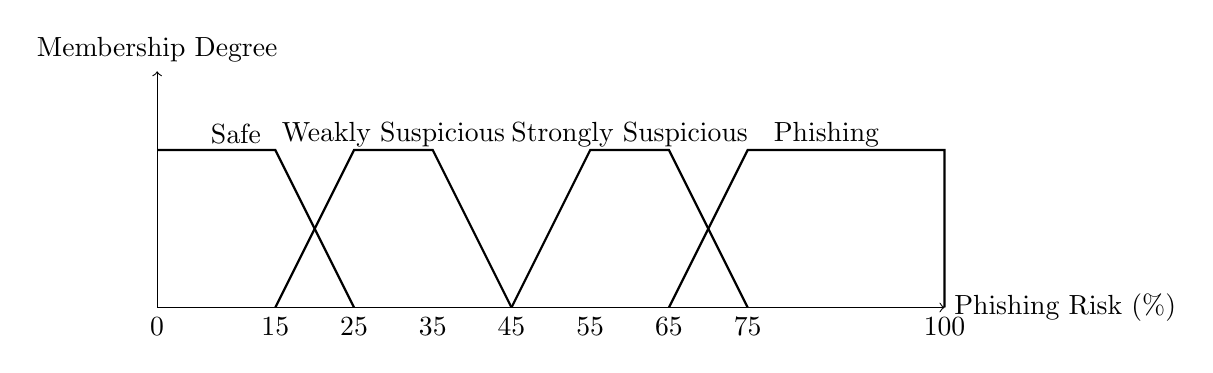
\begin{tikzpicture}
    % Axis
    \draw[->] (0,0) -- (10,0) node[right] {Phishing Risk (\%)};
    \draw[->] (0,0) -- (0,3) node[above] {Membership Degree};

    % Safe
    \draw[thick] (0,2) -- (1.5,2) -- (2.5,0);
    \node at (1,2.2) {Safe};

    % Weakly Suspicious
    \draw[thick] (1.5,0) -- (2.5,2) -- (3.5,2) -- (4.5,0);
    \node at (3,2.2) {Weakly Suspicious};

    % Strongly Suspicious
    \draw[thick] (4.5,0) -- (5.5,2) -- (6.5,2) -- (7.5,0);
    \node at (6,2.2) {Strongly Suspicious};

    % Phishing
    \draw[thick] (6.5,0) -- (7.5,2) -- (10,2) -- (10,0);
    \node at (8.5,2.2) {Phishing};

    % Labels
    \node[below] at (0,0) {0};
    \node[below] at (1.5,0) {15};
    \node[below] at (2.5,0) {25};
    \node[below] at (3.5,0) {35};
    \node[below] at (4.5,0) {45};
    \node[below] at (5.5,0) {55};
    \node[below] at (6.5,0) {65};
    \node[below] at (7.5,0) {75};
    \node[below] at (10,0) {100};
\end{tikzpicture}
\caption{Membership Functions for Phishing Risk}
\label{fig:membership_phishing_risk}
\end{figure}

\section{Task 2: Definition of the Rule Base}\label{sec:task2}

% Define a set of conjunctive rules for the fuzzy expert system.
% - Decide appropriate premises for each rule.
% - Assign a degree of support to each rule.
% - Ensure rules cover all possible combinations of input values.
% - Use rules of different lengths.
% - Avoid inconsistencies and overlaps in the rules.
% - Limit the number of rules to 30-35 for manageability.

\subsection{Rule Development}

The rule base for the fuzzy expert system was developed using a systematic methodology to accurately assess phishing risk while maintaining manageability. Five critical input variables were identified: Ratio of Null Hyperlinks, Number of External CSS Files, Domain Registration Length, Web Traffic, and Page Rank. Each variable was defined with appropriate linguistic terms and membership functions to handle uncertainty. Conjunctive rules were formulated by logically combining these variables' linguistic terms to reflect how different conditions contribute to phishing risk; for example, a high ratio of null hyperlinks and a short domain registration length indicate a potential phishing site. The output variable, Phishing Risk, was specified using linguistic terms ranging from Very Low to Very High based on the expected influence of input conditions. To cover a wide range of scenarios, including both typical cases and edge conditions, the rule set includes rules of varying lengths and complexities, enhancing the system's flexibility and responsiveness. Redundant or conflicting rules were eliminated to maintain the integrity of the rule base. The total number of rules was limited to 35 for manageability.

\subsection{Complete Rule Set}

\begin{table}[H]
    \centering
    \footnotesize
    \setlength{\extrarowheight}{1pt}
    \rowcolors{2}{gray!10}{white}
    \begin{tabularx}{\textwidth}{|>{\centering\arraybackslash}p{0.03\textwidth}|%
    >{\raggedright\arraybackslash}p{0.13\textwidth}|%
    >{\raggedright\arraybackslash}p{0.10\textwidth}|%
    >{\raggedright\arraybackslash}p{0.13\textwidth}|%
    >{\raggedright\arraybackslash}p{0.10\textwidth}|%
    >{\raggedright\arraybackslash}p{0.15\textwidth}|%
    >{\centering\arraybackslash}p{0.08\textwidth}|%
    >{\raggedright\arraybackslash}p{0.12\textwidth}|}
    \hline
    \rowcolor{gray!30}
    \textbf{\#} & \textbf{Null Links} & \textbf{Ext. CSS} & \textbf{Domain Reg.} & \textbf{Traffic} & \textbf{Page Rank} & \textbf{Weight} & \textbf{Risk} \\ \hline
    
    \textbf{1} & High & * & * & * & * & 0.50 & \textbf{Phishing} \\ \hline
    \textbf{2} & Moderate & Few & Short & Very Low & Not Very Known & 0.85 & \textbf{Phishing} \\ \hline
    \textbf{3} & Moderate & Few & Short & Very Low & Moderately Known & 0.85 & \textbf{Phishing} \\ \hline
    \textbf{4} & Moderate & Few & Medium & Very Low & Not Very Known & 0.80 & \textbf{Phishing} \\ \hline
    \textbf{5} & Moderate & Few & Medium & Very Low & Moderately Known & 0.80 & \textbf{Phishing} \\ \hline
    \textbf{6} & Moderate & Normal & Short & Very Low & Not Very Known & 0.75 & \textbf{Phishing} \\ \hline
    \textbf{7} & Moderate & Normal & Short & Very Low & Moderately Known & 0.75 & \textbf{Phishing} \\ \hline
    \textbf{8} & Moderate & Normal & Medium & Very Low & Not Very Known & 0.70 & \textbf{Phishing} \\ \hline
    \textbf{9} & Moderate & Normal & Medium & Very Low & Moderately Known & 0.70 & \textbf{Phishing} \\ \hline
    
    \textbf{10} & * & Very Few & * & * & * & 0.50 & \textbf{Strongly Suspicious} \\ \hline
    \textbf{11} & Moderate & Few & Short & Low & Not Very Known & 0.85 & \textbf{Strongly Suspicious} \\ \hline
    \textbf{12} & Moderate & Few & Short & Low & Moderately Known & 0.85 & \textbf{Strongly Suspicious} \\ \hline
    \textbf{13} & Moderate & Few & Medium & Low & Not Very Known & 0.80 & \textbf{Strongly Suspicious} \\ \hline
    \textbf{14} & Moderate & Few & Medium & Low & Moderately Known & 0.80 & \textbf{Strongly Suspicious} \\ \hline
    \textbf{15} & Moderate & Normal & Short & Low & Not Very Known & 0.75 & \textbf{Strongly Suspicious} \\ \hline
    \textbf{16} & Moderate & Normal & Short & Low & Moderately Known & 0.75 & \textbf{Strongly Suspicious} \\ \hline
    \textbf{17} & Moderate & Normal & Medium & Low & Not Very Known & 0.70 & \textbf{Strongly Suspicious} \\ \hline
    \textbf{18} & Moderate & Normal & Medium & Low & Moderately Known & 0.70 & \textbf{Strongly Suspicious} \\ \hline
    
    \textbf{19} & Moderate & Few & Short & Moderate & Not Very Known & 0.85 & \textbf{Weakly Suspicious} \\ \hline
    \textbf{20} & Moderate & Few & Short & Moderate & Moderately Known & 0.85 & \textbf{Weakly Suspicious} \\ \hline
    \textbf{21} & Moderate & Few & Medium & Moderate & Not Very Known & 0.80 & \textbf{Weakly Suspicious} \\ \hline
    \textbf{22} & Moderate & Few & Medium & Moderate & Moderately Known & 0.80 & \textbf{Weakly Suspicious} \\ \hline
    \textbf{23} & Moderate & Normal & Short & Moderate & Not Very Known & 0.75 & \textbf{Weakly Suspicious} \\ \hline
    \textbf{24} & Moderate & Normal & Short & Moderate & Moderately Known & 0.75 & \textbf{Weakly Suspicious} \\ \hline
    \textbf{25} & Moderate & Normal & Medium & Moderate & Not Very Known & 0.70 & \textbf{Weakly Suspicious} \\ \hline
    \textbf{26} & Moderate & Normal & Medium & Moderate & Moderately Known & 0.70 & \textbf{Weakly Suspicious} \\ \hline
    
    \textbf{27} & * & Few & * & High & * & 0.50 & \textbf{Safe} \\ \hline
    \textbf{28} & Low & * & * & * & * & 0.50 & \textbf{Safe} \\ \hline
    \textbf{29} & * & * & Long & * & * & 0.50 & \textbf{Safe} \\ \hline
    \textbf{30} & * & * & * & * & Popular & 0.50 & \textbf{Safe} \\ \hline
    \textbf{31} & Moderate & Normal & Short & High & Not Very Known & 0.85 & \textbf{Safe} \\ \hline
    \textbf{32} & Moderate & Normal & Short & High & Moderately Known & 0.85 & \textbf{Safe} \\ \hline
    \textbf{33} & Moderate & Normal & Medium & High & Not Very Known & 0.80 & \textbf{Safe} \\ \hline
    \textbf{34} & Moderate & Normal & Medium & High & Moderately Known & 0.80 & \textbf{Safe} \\ \hline
    \textbf{35} & * & Few & * & High & * & 0.50 & \textbf{Safe} \\ \hline
    
    \end{tabularx}
    \caption{Complete Rule Set for Phishing Detection with Weights}
    \label{tab:complete_rule_set}
\end{table} 

\subsection{Rule Set Design Rationale}

The development of our fuzzy rule set was guided by a comprehensive analysis of the practical constraints and resources required for attackers to manipulate various website features. By understanding the cost-benefit relationships from an attacker's perspective, we were able to establish a hierarchy of feature importance and create rules that reflect real-world attack patterns.

Our approach began by analyzing each feature through the lens of attacker constraints, considering the financial costs, technical complexity, and time investments required to manipulate them. This analysis directly influenced how we weighted and combined features in our rule set.

Domain registration length emerged as a significant indicator due to its direct financial implications. Attackers typically aim to minimize operational costs, making long-term domain registrations financially unattractive. Legitimate businesses often register domains for extended periods, while phishing operations tend to use short-term registrations to reduce expenses. However, we recognize that this feature alone is insufficient for classification, as demonstrated by our rules where short registration periods are offset by other positive indicators.

Web traffic presents a more complex scenario for classification. While it can be artificially inflated through various means, including advertising campaigns, bot networks, and embedding techniques, these methods require financial investment. This understanding influenced our rule design, where high traffic alone does not guarantee a safe classification without corroborating positive indicators from other features. Attackers can potentially manipulate traffic through paid advertising or automated tools, making it a valuable but not definitive indicator.

Page rank represents a more resilient metric due to its multifaceted nature. While traffic manipulation can influence page rank, achieving high rankings in search engine results requires sophisticated SEO strategies and sustained effort. The technical expertise and time investment required for SEO manipulation makes this feature particularly valuable in our classification system, especially when combined with other positive indicators.

The ratio of null hyperlinks serves as a crucial technical indicator. Modern web scraping tools like HTTrack \cite{httrack} and GoClone \cite{goclone} can easily copy website structures, but often result in broken or placeholder links (\textit{href="\#"}). This pattern emerges when attackers hastily replicate legitimate sites without properly maintaining link functionality. Our rules heavily weight this feature, as high ratios of null hyperlinks strongly suggest automated copying typical of phishing attempts.

External CSS file count provides insight into website development practices. While tools can copy entire CSS files, maintaining multiple external stylesheets represents a level of development sophistication typically associated with legitimate websites. Phishing sites often consolidate CSS to simplify deployment, making the number of external stylesheets a useful discriminator between legitimate and malicious sites.

These understandings directly shaped our rule set structure. High-risk classifications (Phishing) typically require multiple high-cost negative indicators, such as a high ratio of null hyperlinks combined with short domain registration and very few CSS files. Moderate-risk classifications (Strongly Suspicious) often involve mixed signals, where some high-cost features appear legitimate while others show suspicious patterns. Low-risk classifications (Safe) generally require multiple positive indicators that would be costly or time-consuming for attackers to fake simultaneously.

\section{Task 3: Implementation Using MATLAB Fuzzy Toolkit}

% Describe the implementation of the fuzzy expert system in MATLAB.
% - Specify the use of min as t-norm and max as t-conorm.
% - Use Center of Area for defuzzification.
% Validate the system using 3D plots of the rules.

Following the approach defined throughout the previous sections, the Fuzzy Expert System was implemented using \textit{MATLAB's Fuzzy Logic Designer Toolkit}. We defined five input variables and one output variable, each with their respective membership functions, modeled using the trapezoidal functions detailed in Section \ref{sec:task1}. Additionally, we constructed the full set of 35 rules described in Section \ref{sec:task2}, ensuring comprehensive coverage of the system’s logic.

Our implementation employs the \textit{minimum} (min) operator as the t-norm for conjunctions and the \textit{maximum} (max) operator as the t-conorm for disjunctions. These operators are selected to ensure consistency with standard fuzzy logic principles while maintaining computational simplicity.

For defuzzification, we utilized the \textit{Center of Area} (CoA) method, as it provides a precise and interpretable output. This method calculates the centroid of the aggregated fuzzy set to generate the crisp output value, ensuring a balanced representation of all contributing rules.

We validated the system using 3D surface plots generated by MATLAB's visualization tools. These plots depict the relationships between input variables and the output, offering a clear representation of how the defined rules influence the system's behavior. This step verified the correctness of the rule base and the effectiveness of the membership functions.

\subsection{System Configuration}

% Explain how the fuzzy inference system was set up in MATLAB.
% Include screenshots if necessary.

The fuzzy inference system was set up using MATLAB's \textit{Fuzzy Logic Designer Toolkit} with the following configuration:

\begin{itemize}
    \item \textbf{Type}: Mamdani Type-1
    \item \textbf{Input Variables}: 5  
    \begin{itemize}
        \item Ratio of Null Hyperlinks
        \item Number of External CSS
        \item Domain Registration Length
        \item Web Traffic
        \item Page Rank
    \end{itemize}
    \item \textbf{Output Variable}: Phishing Risk
    \item \textbf{Membership Functions}:  
    \begin{itemize}
        \item Each input variable is modeled with \textbf{3 or 4 membership functions} using trapezoidal shapes.
        \item The output variable is modeled with \textbf{4 membership functions}.
    \end{itemize}
    \item \textbf{Rule Base}: A total of \textbf{35 rules} were defined.
    \item \textbf{Operators}:  
    \begin{itemize}
        \item \textit{AND Method}: Minimum (t-norm)
        \item \textit{OR Method}: Maximum (t-conorm)
        \item \textit{Implication Method}: Minimum
        \item \textit{Aggregation Method}: Maximum
    \end{itemize}
    \item \textbf{Defuzzification Method}: Center of Area (centroid)
\end{itemize}

The configuration and connections between the variables are illustrated in Figure \ref{fig:system_configuration}.
\begin{figure}[H]
    \centering
    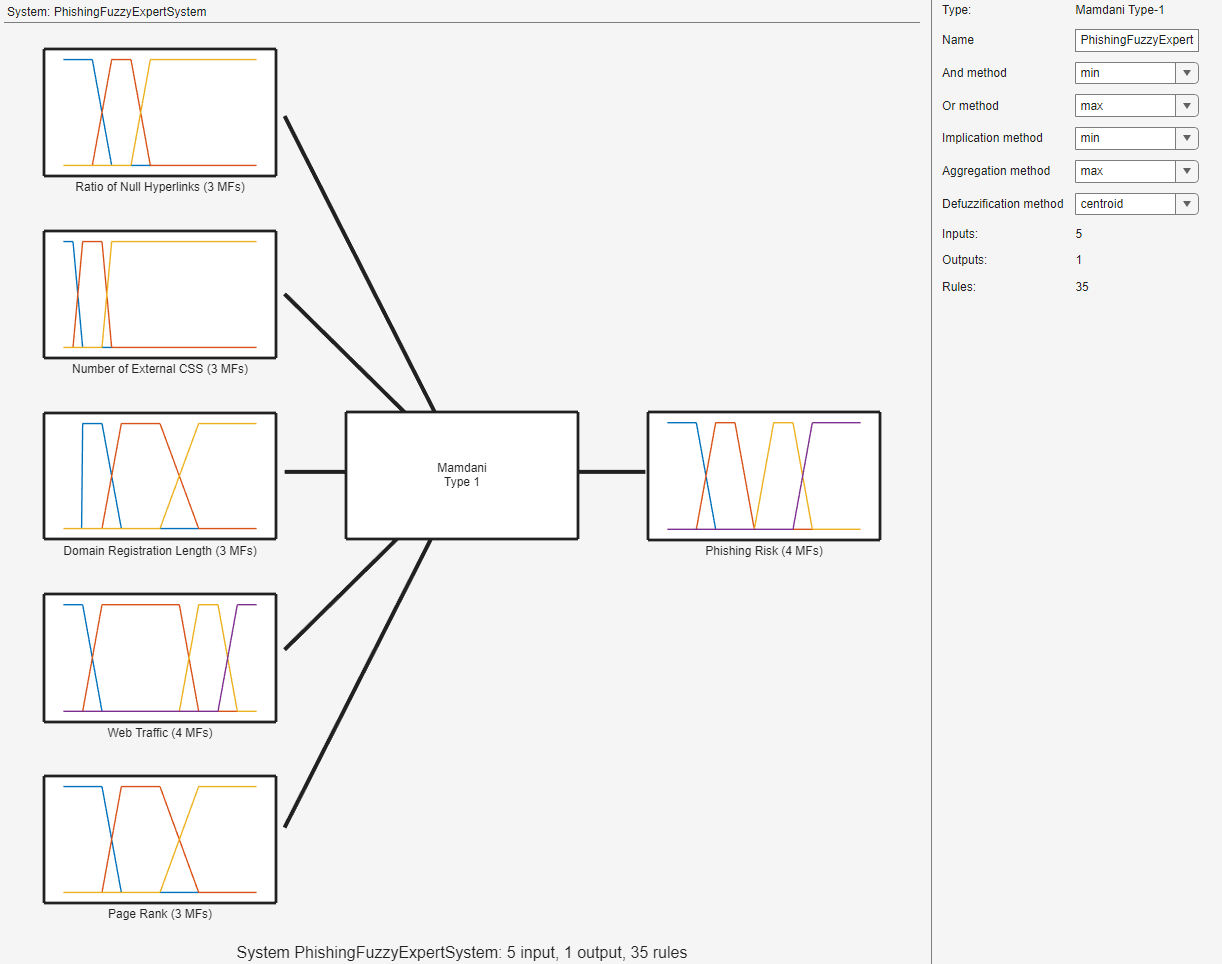
\includegraphics[width=0.8\textwidth]{figures/SystemConfiguration.png}
    \caption{System Configuration in MATLAB's Fuzzy Logic Designer Toolkit}
    \label{fig:system_configuration}
\end{figure}

\subsection{Validation}

% Present the 3D plots.
% Discuss how they validate the system's behavior.

The validation of the fuzzy expert system was performed using the 3D Control Surface plots generated by the Fuzzy Logic Designer Toolkit, which depict the output variable (\textit{Phishing Risk}) as a function of two input variables at a time. These plots are generated based on the defined set of 35 rules.

Several 3D plots were analyzed, each illustrating the relationship between different pairs of input variables and the output. An important argument validating the system's behavior is that the resulting surfaces exhibit \textbf{monotonicity}. This indicates that the output (\textit{Phishing Risk}) consistently increases or decreases as the input variables change, aligning with expectations based on the rule base.

Four of these 3D plots are presented in Figure \ref{fig:3d_plots} for visualization.  

\begin{figure}[H]
    \centering
    % Replace with actual plot file names
    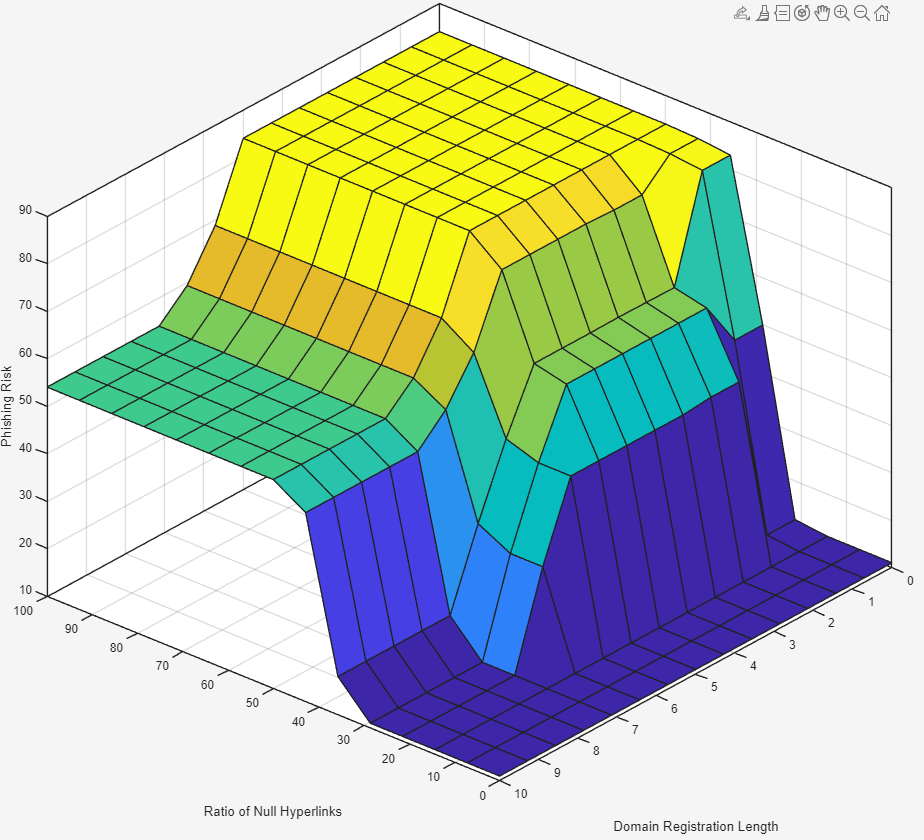
\includegraphics[width=0.49\textwidth]{figures/Surface_NullLinks_DomainReg.png}
    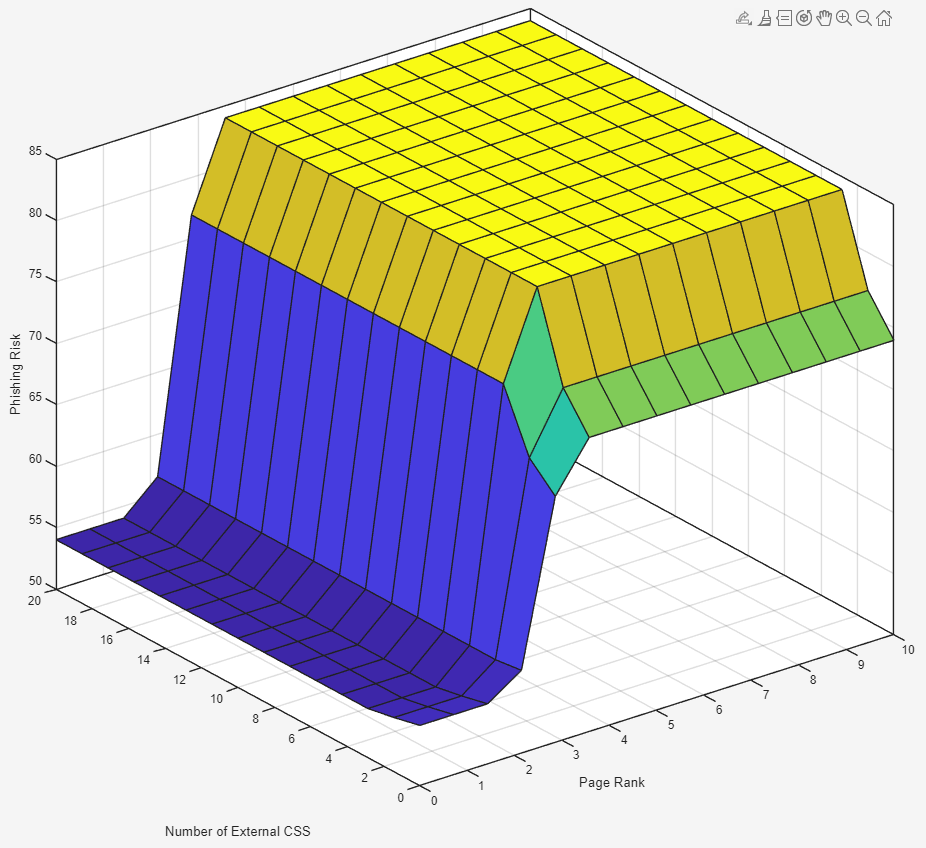
\includegraphics[width=0.49\textwidth]{figures/Surface_CSS_PageRank.png}
    \\
    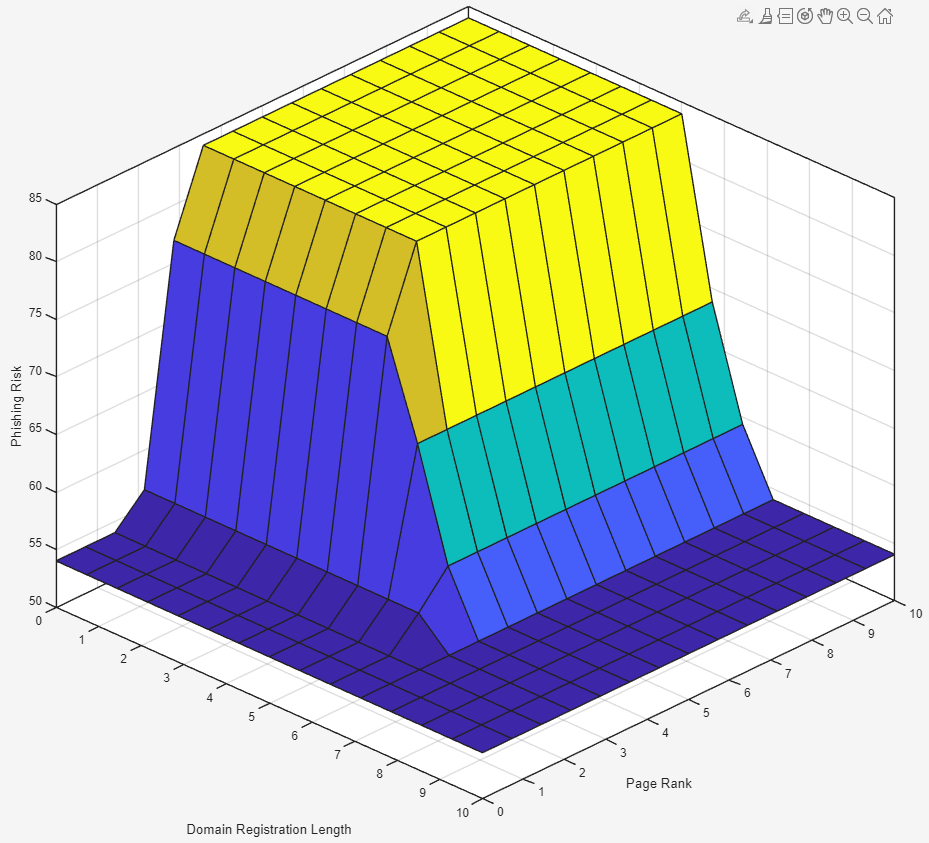
\includegraphics[width=0.49\textwidth]{figures/Surface_PageRank_DomainReg.png}
    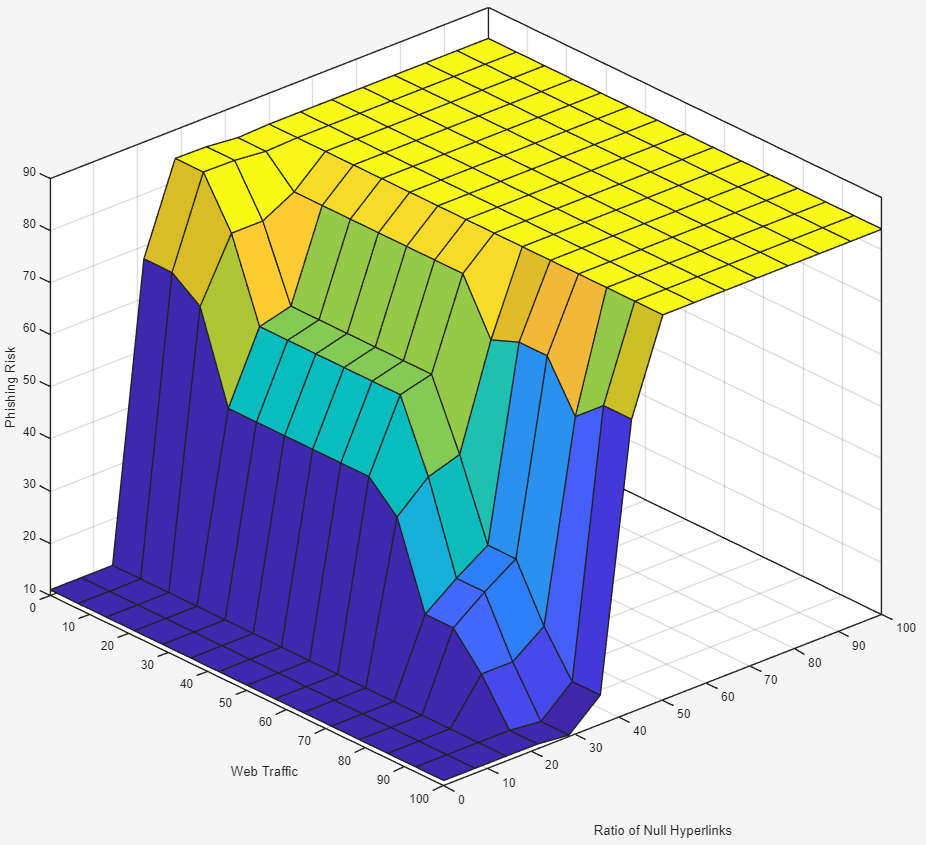
\includegraphics[width=0.49\textwidth]{figures/Surface_WebTraffic_NullLinks.png}
    \caption{3D surface plots of the output variable as a function of input variable pairs.}
    \label{fig:3d_plots}
\end{figure}

\section{Task 4: Testing the System}

% Test the fuzzy expert system with four different websites.
% - Select or invent appropriate test cases representing different situations.
% - Ensure some cases activate more than one label of the same variable.
% Report the results with explanations and screenshots.

To evaluate the performance and reliability of the fuzzy expert system, we conducted tests using four different websites. These test cases were carefully created to represent various scenarios, ensuring a diverse range of inputs and outputs. The objective was to analyze the system's behavior under different conditions and validate that the output aligns with expectations.

Each test case includes specific input values for the five input variables, with some cases intentionally designed to activate more than one membership label for the same variable. This approach ensures the system utilizes multiple rules to compute the output (\textit{Phishing Risk}), demonstrating the effectiveness of the rule base and inference mechanism.

\subsection{Test Cases}

% Describe each test case in detail.
% Include input values and expected outcomes.

The following test cases describe the input values and expected outcomes for the fuzzy expert system:

\begin{itemize}
    \item \textbf{Test Case 1: Legitimate Website}
    
    This case represents a legitimate website with benign characteristics. The input values were selected to reflect a low likelihood of phishing activity:
    \begin{itemize}
        \item \textit{Ratio of Null Hyperlinks}: 5\%
        \item \textit{Number of External CSS}: 15 files
        \item \textit{Domain Registration Length}: 8 years
        \item \textit{Web Traffic}: 85-th percentile
        \item \textit{Page Rank}: 2.5 popularity score
    \end{itemize}
    \textbf{Expected Outcome:} Low \textit{Phishing Risk}.
    
    \item \textbf{Test Case 2: Suspicious Website}
    
    This case simulates a borderline suspicious website with mixed indicators:
    \begin{itemize}
        \item \textit{Ratio of Null Hyperlinks}: 40\%
        \item \textit{Number of External CSS}: 3 files
        \item \textit{Domain Registration Length}: 4 years
        \item \textit{Web Traffic}: 65-th percentile
        \item \textit{Page Rank}: 4.8 popularity score
    \end{itemize}
    \textbf{Expected Outcome:} Medium \textit{Phishing Risk}.

    \item \textbf{Test Case 3: Phishing Website}
    
    This case reflects a highly suspicious phishing website with characteristics strongly indicative of phishing activity:
    \begin{itemize}
        \item \textit{Ratio of Null Hyperlinks}: 85\%
        \item \textit{Number of External CSS}: 1 file
        \item \textit{Domain Registration Length}: 1 year
        \item \textit{Web Traffic}: 18-th percentile
        \item \textit{Page Rank}: 8.2 popularity score
    \end{itemize}
    \textbf{Expected Outcome:} High \textit{Phishing Risk}.
    
    \item \textbf{Test Case 4: Ambiguous Website}
    
    This case represents an ambiguous website with conflicting indicators that activate multiple rules:
    \begin{itemize}
        \item \textit{Ratio of Null Hyperlinks}: 50\%
        \item \textit{Number of External CSS}: 2 files
        \item \textit{Domain Registration Length}: 6 years
        \item \textit{Web Traffic}: 80-th percentile
        \item \textit{Page Rank}: 2.1 popularity score
    \end{itemize}
    \textbf{Expected Outcome:} Medium \textit{Phishing Risk}.
\end{itemize}

\subsection{Results and Discussion}

% Present the outputs of the system for each test case.
% Show activations of rules and explain the results.

The following results demonstrate the system's behavior for each of the test cases. Rules activated during the inference process and the corresponding \textit{Phishing Risk} outputs are presented for each case.  

\begin{itemize}
    \item \textbf{Test Case 1: Legitimate Website}
    \begin{itemize}
        \item \textit{Rules activated:} 28, 29, 30
        \item \textit{Phishing risk:} 11.0 (Safe)
    \end{itemize}
    \begin{figure}[H]
        \centering
        % Replace with actual plot file names
        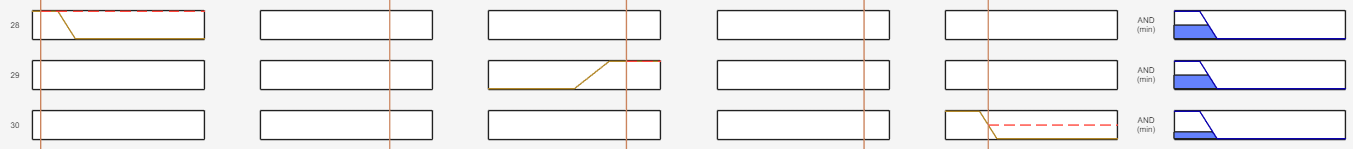
\includegraphics[width=0.99\textwidth]{figures/Activations_Test1.png}
        \\
        \hfill
        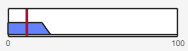
\includegraphics[width=0.20\textwidth]{figures/Output_Test1(11).png}
        \caption{Rules activation and output for Test Case 1.}
        \label{fig:test1}
    \end{figure}
    For this case, the system activated rules 28, 29, and 30, which primarily correspond to input variables indicating a low risk of phishing. The resulting \textit{Phishing Risk} value is \textbf{11.0}, categorizing the website as \textit{Safe}. The surface plot confirms the expected behavior, as all inputs align with low-risk labels.  

    \item \textbf{Test Case 2: Suspicious Website}
    \begin{itemize}
        \item \textit{Rules activated:} 1, 14, 22
        \item \textit{Phishing risk:} 55.3 (Strongly suspicious)
    \end{itemize}    
    \begin{figure}[H]
        \centering
        % Replace with actual plot file names
        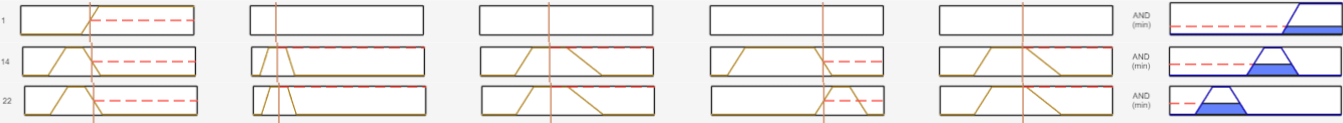
\includegraphics[width=0.99\textwidth]{figures/Activations_Test2.png}
        \\
        \hfill
        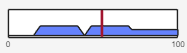
\includegraphics[width=0.20\textwidth]{figures/Output_Test2(55-3).png}
        \caption{Rules activation and output for Test Case 2.}
        \label{fig:test2}
    \end{figure}
    Here, rules 1, 14, and 22 were activated, reflecting medium input values for various variables. The output \textit{Phishing Risk} is \textbf{55.3}, categorizing the website as \textit{Strongly Suspicious}. This result is consistent with the rule base, where medium risk variables combine to produce a moderately high output.  

    \item \textbf{Test Case 3: Phishing Website}
    \begin{itemize}
        \item \textit{Rules activated:} 1, 10
        \item \textit{Phishing risk:} 74.0 (0.1 Strongly suspicious, 0.9 Phishing)
    \end{itemize}    
    \begin{figure}[H]
        \centering
        % Replace with actual plot file names
        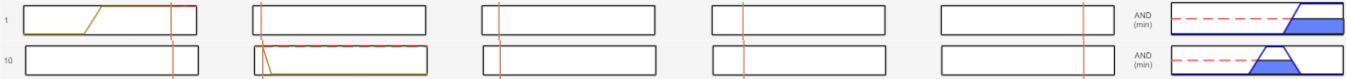
\includegraphics[width=0.99\textwidth]{figures/Activations_Test3.png}
        \\
        \hfill
        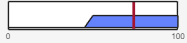
\includegraphics[width=0.20\textwidth]{figures/Output_Test3(74).png}
        \caption{Rules activation and output for Test Case 3.}
        \label{fig:test3}
    \end{figure}
    In this case, rules 1 and 10 were triggered, primarily due to high-risk indicators across all input variables. The system computed a \textit{Phishing Risk} of \textbf{74.0}, mostly categorizing the website as \textit{Phishing}. The activation of high-risk membership functions and rules aligns with expectations, as the inputs strongly suggest phishing activity.  

    \item \textbf{Test Case 4: Ambiguous Website}
    \begin{itemize}
        \item \textit{Rules activated:} 1, 29, 30
        \item \textit{Phishing risk:} 55.7 (Strongly suspicious)
    \end{itemize}    
    \begin{figure}[H]
        \centering
        % Replace with actual plot file names
        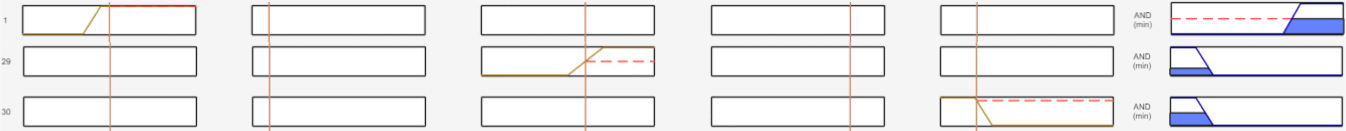
\includegraphics[width=0.99\textwidth]{figures/Activations_Test4.png}
        \\
        \hfill
        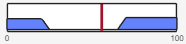
\includegraphics[width=0.20\textwidth]{figures/Output_Test4(55-7).png}
        \caption{Rules activation and output for Test Case 4.}
        \label{fig:test4}
    \end{figure}
    For this ambiguous case, rules 1, 29, and 30 were activated. The inputs include both high and low-risk indicators, leading to a \textit{Phishing Risk} of \textbf{55.7}. The output categorizes the website as \textit{Strongly Suspicious}. This result highlights the system's ability to handle conflicting inputs, as multiple rules contribute to the final output.
    
\end{itemize}

\section{Task 5: Design of an Enhanced Fuzzy Expert System}

% Question: How to visualize this?
% Propose a design for a more comprehensive fuzzy expert system.
% - Include more features about websites.
% - Illustrate inputs, outputs, and rule blocks in a diagram.
% Note: No specific variable definitions or rules are required.

\subsection{Proposed System Architecture}

% Describe the proposed enhancements and their benefits.
% Include a figure illustrating the system.

\section{Conclusion}

% Summarize the work done.
% Reflect on the effectiveness of the fuzzy expert system.
% Discuss potential improvements and future work.

% \appendix

\printbibliography

\end{document}